\documentclass{beamer} 
\usetheme{default} 
\setbeamercovered{transparent}

%\useoutertheme{umbcfootline} 
\setbeamertemplate{background canvas}[vertical shading][bottom=red!20,top=yellow!30] 


\usepackage[spanish]{babel}
%\usepackage[latin1]{inputenc}
\usepackage[utf8x]{inputenc}
\usepackage{multicol}
%\usepackage{color}
\usepackage[usenames,dvipsnames]{color}
\title{Interfaces en java}

\author{Manuel J. Molino Milla \and Luis Molina Garzón}

\date{\today} %

\institute{IES Virgen del Carmen \and Departamento de Informática}




%\beamerdefaultoverlayspecification{<+->}

\begin{document}


\begin{frame}
  \titlepage
\end{frame}

\begin{frame}
    \frametitle{Logo}
\begin{figure}
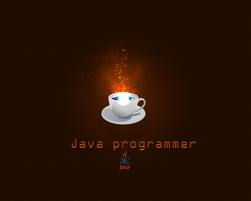
\includegraphics[scale=1]{imagenes/logo.jpeg} 
\caption{Logo Java}
\end{figure}
\end{frame}

%\begin{frame}
 % \frametitle{Contenido}
 %\tableofcontents[pausesections]
%\end{frame}




\begin{frame}[fragile]
\frametitle{Introducción a las clases abstractas}
\begin{small}
\begin{itemize}[<+->]
\item Hay ocasiones, cuando se desarrolla una jerarquía de clases en que algún comportamiento está presente en todas ellas pero se materializa de forma distinta para cada una.
\item Por ejemplo, pensemos en una estructura de clases para manipular figuras geométricas.
\item Podríamos pensar en tener una clase genérica, que podría llamarse FiguraGeometrica y una serie de clases que extienden a la anterior que podrían ser Circulo, Poligono,\dots
\item Podría haber un método dibujar dado que sobre todas las figuras puede llevarse a cabo esta acción.
\item Pero las operaciones concretas para llevarla a cabo dependen del tipo de figura en concreto (de su clase).
\item Por otra parte la acción dibujar no tiene sentido para la clase genérica FiguraGeometrica, porque esta clase representa una abstracción del conjunto de figuras posibles.
\item Para resolver esta problemática Java proporciona las clases y métodos abstractos
\end{itemize}
\end{small}
\end{frame}

\begin{frame}[fragile]
\frametitle{Ejemplo}
\begin{scriptsize}
\begin{verbatim}
abstract class FiguraGeometrica {
    . . .
    abstract void dibujar();
    . . .
}

class Circulo extends FiguraGeometrica {
    . . .
    void dibujar() {
        // codigo para dibujar Circulo
        . . .
    }
} 
\end{verbatim}
\pause
\begin{itemize}[<+->]
\item  Un método abstracto es un método declarado en una clase para el cual esa clase no proporciona la implementación (el código).
\item Una clase abstracta es una clase que tiene al menos un método abstracto.
\item Una clase que extiende de una clase abstracta debe implementar los métodos abstractos (escribir el código)
\item O bien volverlos a declarar como abstractos, con lo que ella misma se convierte también en clase abstracta. 
\end{itemize}
\end{scriptsize}
\end{frame}

 
\begin{frame}[fragile]
\frametitle{Referencias y objetos abstractos}
\begin{itemize}[<+->]
\item Se pueden crear referencias a clases abstractas como cualquier otra.
\item No hay ningún problema en poner: \emph{FiguraGeometrica figura;}
\item Sin embargo una clase abstracta no se puede instanciar, es decir, no se pueden crear objetos de una clase abstracta. 
\item El compilador producirá un error si se intenta:
\item \emph{FiguraGeometrica figura = new FiguraGeometrica();}
\item Sin embargo utilizando el \textbf{up-casting}: 
\item \emph{FiguraGeometrica figura = new Circulo(\dots); figura.dibujar();}
\end{itemize}
\end{frame}

\begin{frame}[fragile]
\frametitle{Ejemplo}
\begin{figure}
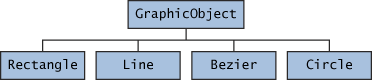
\includegraphics[scale=0.5]{imagenes/abstract1.png}
\end{figure}
\begin{tiny}
\begin{multicols}{2}
\begin{verbatim}
abstract class GraphicObject {
    int x, y;
    ...
    void moveTo(int newX, int newY) {
        ...
    }
    abstract void draw();
    abstract void resize();
}







class Circle extends GraphicObject {
    void draw() {
        ...
    }
    void resize() {
        ...
    }
}
class Rectangle extends GraphicObject {
    void draw() {
        ...
    }
    void resize() {
        ...
    }
}
\end{verbatim}
\end{multicols}
\end{tiny}
\end{frame}



\begin{frame}[fragile]
\frametitle{Caracteristicas de las clases abstractas}
\begin{footnotesize}
\begin{itemize}[<+->]
\item Que una clase abstracta no pueda ser instanciada no implica que no pueda tener un constructor.
\item Si no definimos un constructor, existe el constructor por defecto.
\item El sentido del constructor en las clases abstractas obliga a \emph{settear} los valores de los atributos de la clase base (clase abstracta).
\end{itemize}
\end{footnotesize}
\pause
\begin{tiny}
\begin{verbatim}
        public abstract class FiguraGeometrica
         {
           private String nombre;
           public abstract double area ();

         public FiguraGeometrica (String nombre)
           {
             this.nombre = nombre;
           }
         public String toString ()
           {
             return this.nombre + " area: " + this.area ();
           }
         public String getNombre ()
           {
             return this.nombre;
           }
         public void setNombre (String nombre)
           {
             this.nombre = nombre;
           }
         }    
\end{verbatim}
\end{tiny}
\end{frame}

\begin{frame}[fragile]
\frametitle{Siguiendo el ejemplo}
\begin{multicols}{2}
\begin{tiny}
\begin{verbatim}







import java.lang.Math;
public class Circulo extends FiguraGeometrica
{
  private int radio;
  public Circulo (int r)
  {
    super ("Círculo");
    this.radio = r;
  }
  public double area ()
  {
    return Math.PI * radio * radio;
  }
}







public class Cuadrado extends FiguraGeometrica
{
  private int arista;
  public Cuadrado (int a)
  {
    super ("Cudrado");
    this.arista = a;
  }
  public double area ()
  {
    return arista * arista;
  }
}


public class TestFiguraGeometricas
{
  public static void main (String[]arg)
  {
    Circulo c = new Circulo (2);
    System.out.println ("Figura: " + c.getNombre ());
    System.out.println ("Área: " + c.area ());
    Cuadrado cu = new Cuadrado (2);
    System.out.println ("Figura: " + cu.getNombre ());
    System.out.println ("Área: " + cu.area ());
  }
}

\end{verbatim}
\end{tiny}
\end{multicols}
\end{frame}

\begin{frame}
\frametitle{Interfaces}
\begin{itemize}[<+->]
\item Una interfaz es similar a las clases abstractas.
\item Establece la apariencia que tendrán todas las clases que \textbf{implementen} esa interfaz.
\item Permite al creador establecer la forma de una clase: \emph{nombres de metodos, listas de parametros, y tipos de retorno, pero no cuerpos de metodo.}
\item Una interfaz tambien puede tener campos, peros estos son implicitamente \textbf{estaticos y constantes}.
\item Para crear una interfaz usamos la palabra \alert{interface} en vez de \textbf{class}.
\item Para hacer que una clase se ajuste a una interfaz particular se usa la palabra clave \alert{implements}.
\item Mientras que la herencia una clase \textbf{solo} puede tener \textbf{una} clase padre, en este caso una clase puede implementar \textbf{varias} interfaces
\end{itemize}
\end{frame}



\begin{frame}[fragile]
\frametitle{Interfaces}
Una interface se declara:
{\color{blue}
\begin{verbatim}
interface nombre_interface {
    tipo_retorno nombre_metodo ( lista_argumentos ) ;
    . . . 
}
\end{verbatim}}
\pause
Por ejemplo:
\begin{footnotesize}
{\color{blue}
\begin{verbatim}
interface InstrumentoMusical {
    void tocar();
    void afinar();
    String tipoInstrumento();
}
\end{verbatim}}
\end{footnotesize}
\pause
Y una clase que implementa la interface:
\begin{scriptsize}
{\color{blue}
\begin{verbatim}
class InstrumentoViento implements InstrumentoMusical {
      void tocar() { . . . };
      void afinar() { . . .};
      String tipoInstrumento() {}
}
class Guitarra extends InstrumentoViento {
      String tipoInstrumento() {
      return "Guitarra";
      }
}   
\end{verbatim}}
\end{scriptsize}
\end{frame}


\begin{frame}[fragile]
\frametitle{Referencias a Interfaces}
Es posible crear referencias a interfaces, pero las interfaces no pueden ser instanciadas. Una referencia a una interface puede ser asignada a cualquier objeto que implemente la interface. Por ejemplo:
{\color{magenta}
\begin{verbatim}
InstrumentoMusical instrumento = new Guitarra();
instrumento.play();
System.out.prinln(instrumento.tipoInstrumento());

//error.No se puede instanciar:
InstrumentoMusical i2 = new InstrumentoMusical(); 
\end{verbatim}}
\end{frame}

\begin{frame}[fragile]
\frametitle{Extensión de interfaces}
Las interfaces pueden extender otras interfaces y, a diferencia de las clases, una interface puede extender más de una interface. La sintaxis es:
{\color{cyan}
\begin{verbatim}
interface nombre_interface  extends nombre_interface, ...{
    tipo_retorno nombre_metodo ( lista_argumentos ) ;
    . . . 
}
\end{verbatim}}
\end{frame}


\begin{frame}[fragile]
\frametitle{Agrupaciones de constantes}
{\color{purple}
\begin{verbatim}
public interface Meses {
 int ENERO = 1 , FEBRERO = 2 . . . ;
 String [] NOMBRES_MESES = { " " , "Enero", "Febrero",...};
}
\end{verbatim}}
\pause
Esto puede usarse simplemente:
{\color{purple}
\begin{verbatim}
System.out.println(Meses.NOMBRES_MESES[ENERO]);
\end{verbatim}}
\end{frame}

\begin{frame}[fragile]
\frametitle{Cosas importantes sobre interfaces}
\begin{itemize}[<+->]
\item     Todos los métodos de una interfaz son implícitamente \textbf{public abstract}, no es necesario especificarlo en la declaración del mismo.
\item  Todas las variables y atributos de una interfaz son implícitamente constantes (\textbf{public static final}), no es necesario especificarlo en la declaración del misma
\item  Los métodos de una interfaz no pueden ser: static o final.
\item  Una interfaz puede heredar (\textbf{extends}) de una o más interfaces.
\item  Una interfaz \textbf{no} puede heredar de otro elemento que no sea una interfaz.
\item  Una interfaz no puede implementar (\textbf{implements}) otra interfaz.
\item  Una interfaz debe ser declarada con la palabra clave \textbf{interface}.
\item  Una interfaz puede ser public o package (valor por defecto). 
\end{itemize}

\end{frame}



\begin{frame}[fragile]
\frametitle{Interfaz Comparable}
El código de esta interfaz es
\begin{verbatim}
package java.lang;
public interface Comparable<T>{
  public int compareTo(T obj);
}
\end{verbatim}
\begin{itemize}[<+->]
\item Define un unico metodo \emph{CompareTo}
\item Recibe como parametro un objeto generico.
\item Retorna un entero.
\item Este puede ser mayor, menor o igual que cero.
\item Dependiendo de la comparacion de los atributos del objeto \emph{this} y los del objeto que se pasa como paramentro \emph{Obj}
\item Ejemplo:
\end{itemize}
\end{frame}

\begin{frame}[fragile]
\frametitle{Ejemplo}
\begin{footnotesize}
\begin{verbatim}
public class Actor implements Comparable < Actor >
{
  private String nombre;
  private int numeroPeliculas;
  public Actor (String nombre, int numeroPeliculas)
  {
    this.nombre = nombre;
    this.numeroPeliculas = numeroPeliculas;
  }
  public int compareTo (Actor otroActor)
  {
    return this.numeroPeliculas - otroActor.numeroPeliculas;
  }
  public static void main (String[]arg)
  {
    Actor a1 = new Actor ("Juan", 12);
    Actor a2 = new Actor ("Pedro", 13);
    System.out.println (a1.compareTo (a2));
    System.out.println (a2.compareTo (a1));
    System.out.println (a1.compareTo (a1));
  }
}
\end{verbatim}
\end{footnotesize}
\end{frame}


\begin{frame}
\frametitle{Importante}
{\LARGE La principal diferencia entre interface y abstract es que un interface proporciona un mecanismo de encapsulación de los protocolos de los métodos sin forzar al usuario a utilizar la herencia.}
\end{frame}

\begin{frame}
\begin{figure}

\includegraphics[scale=0.4]{imagenes/end.png}
\end{figure}
\end{frame}


\end{document}